

\chapter{Laser-based Orientation}
In this...

\section{Projections}
The use of some regular and known geometrical shape that could be projected onto the net for use for orientation 
was early put forward. The idea behind this is based on the work by \citet{carlsen10}, who used 
a set of line lasers for \todo{Hva var dette egentlig?}

\section{Patterns}
There are many different patterns that may give more information about 
orientation of the ROV relative to the net than some simple lines. The 
different polygons in figure \vref{fig:pattern_triangle} to \vref{fig:pattern_heptagon}
were chosen as a good start for further investigation together with the 
circle as shown in \vref{fig:pattern_circle}.

\begin{figure}[htbp]
	\subfloat[Triangle]{
		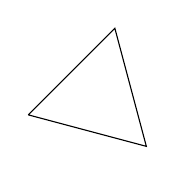
\begin{tikzpicture}[scale=0.1]
			\draw (0,4) -- (11,15) -- (15,0) -- (0,4);
		\end{tikzpicture}\label{fig:pattern_triangle}
	}\hfill
	\subfloat[Square]{
		\begin{tikzpicture}[scale=0.1]
			\draw (0,0) -- (0,15) -- (15,15) -- (15,0) -- (0,0);
		\end{tikzpicture}
	}\hfill
	\subfloat[Pentagon]{
		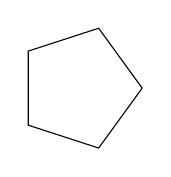
\begin{tikzpicture}[scale=1]
			\newdimen\R
			\R=0.8cm
			\draw (0:\R)
				\foreach \x in {72,144,...,360} {  -- (\x:\R) };
		\end{tikzpicture}
	}\hfill
	\subfloat[Hexagon]{
		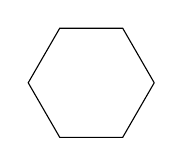
\begin{tikzpicture}[scale=1]
			\newdimen\R
			\R=0.8cm
			\draw (0:\R)
				\foreach \x in {60,120,...,360} {  -- (\x:\R) };
		\end{tikzpicture}
	}\hfill
	\subfloat[Heptagon]{
		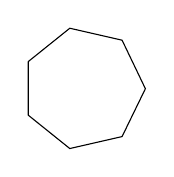
\begin{tikzpicture}[scale=0.8]
			\draw (-0.76,1.54) -- (-0.76,0.69) -- (-0.10,0.16) -- (0.73,0.35) -- (1.1,1.11) -- (0.73,1.88) -- (-0.10,2.07) -- (-0.76,1.54);
		\end{tikzpicture}\label{fig:pattern_heptagon}
	}\hfill
	\subfloat[Circle]{
		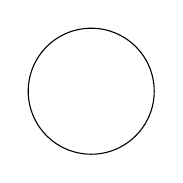
\begin{tikzpicture}[scale=0.8]
			\draw (0,0) circle(1);
		\end{tikzpicture}\label{fig:pattern_circle}
	}\hfill
	\caption{Different laser patterns}
	\label{fig:laser_pattern}
\end{figure}

Criteria for a good pattern should contain
\begin{enumerate}
	\item Not ambiguous when interpolating lines
	\item Easy algorithm to reconstruct shape
	\item Keep orientation information\footnote{Avoid apperture problem, see section \vref{sec:apperture.problem}}
\end{enumerate}

It can be shown that amongst the patterns in figure \vref{fig:laser_pattern} that all patterns with a even number 
of vertices is prone to the apperture problem. 
